%=======================================================================
%  Synthetic Augmentation for Rare-Scenario Football xG:
%  Cross-Competition Cold-Start Transfer and the Instability of
%  Single-Split Method Comparisons
%  IEEE conference format, 6-page limit including references
%
%  FIGURES (4, all single-column, real PNGs in figures/):
%    fig_loco_pipeline_diagram.png   LOCO study-design schematic
%    fig_splitdist_ctgan_smote.png   8-split CTGAN-vs-SMOTE paired plot
%    fig_loco_per_fold.png           LOCO per-competition forest plot (5% ratio)
%    fig_loco_dose_response.png      LOCO six-ratio dose-response
%  Generated by 23_revision_figures.py from results/*.csv.
%
%  TABLES (2): I  eight-split aggregate (incl. Brier)
%              II LOCO per-fold (B_G, Model N, C_G)
%  (The former Table III experimental manifest was folded into one sentence
%  in Methodology; Fig. 1 carries the split-scope information.)
%
%  NOTE (kept out of the paper body for space): CTGAN batch size is
%  min(500, floor(n/2)) rounded down to the nearest multiple of ten, where n
%  is the scope's rare-shot count. Realized values are 470-500 across all
%  folds/splits used here (<=6% variation). See matchgrouped_utils.py.
%=======================================================================
\documentclass[conference,a4paper]{IEEEtran}
\IEEEoverridecommandlockouts
\usepackage[utf8]{inputenc}
\usepackage[T1]{fontenc}
\usepackage{cite}
\usepackage{amsmath,amssymb,amsfonts}
\usepackage{algorithmic}
\usepackage{graphicx}
\graphicspath{{figures/}}
\usepackage{textcomp}
\usepackage{xcolor}
\usepackage{booktabs}
\usepackage{url}
\usepackage{microtype}
\renewcommand{\topfraction}{0.92}
\renewcommand{\bottomfraction}{0.85}
\renewcommand{\textfraction}{0.06}
\renewcommand{\floatpagefraction}{0.72}
\setcounter{topnumber}{3}
\setcounter{bottomnumber}{2}
\setcounter{totalnumber}{4}
\renewcommand{\arraystretch}{0.92}
\setlength{\tabcolsep}{4pt}
\setlength{\abovedisplayskip}{3pt plus 1pt minus 1pt}
\setlength{\belowdisplayskip}{3pt plus 1pt minus 1pt}
\setlength{\abovedisplayshortskip}{2pt plus 1pt minus 1pt}
\setlength{\belowdisplayshortskip}{2pt plus 1pt minus 1pt}
\def\BibTeX{{\rm B\kern-.05em{\sc i\kern-.025em b}\kern-.08em
    T\kern-.1667em\lower.7ex\hbox{E}\kern-.125emX}}

\begin{document}

% Title set at \large rather than IEEEtran's default \huge to reclaim
% vertical space at the top of page 1 (Block 5).
\title{\large Synthetic Augmentation for Rare-Scenario Football xG: Cross-Competition Cold-Start Transfer and the Instability of Single-Split Method Comparisons}

%\author{
%\IEEEauthorblockN{
%\textsuperscript{1}Md. Ashiqur Rahman Abir,
%\textsuperscript{2}Shahzalal Khan Rahat,
%\textsuperscript{3}Mahejabin Yesmin,
%\textsuperscript{4}Farhan Faruk,\\
%\textsuperscript{5}Nafiz Imtiaz Rafin,
%\textsuperscript{6}Md. Golam Rabiul Alam,
%\textsuperscript{7}Zia Uddin
%}

%\IEEEauthorblockA{
%\textsuperscript{1,2,3,4,5,6}
%Department of Computer Science and Engineering,
%BRAC University\\
%Dhaka, Bangladesh
%}

%\IEEEauthorblockA{
%\textsuperscript{7}
%Sustainable Communication Technologies,
%SINTEF Digital\\
%Oslo, Norway
%}

%\IEEEauthorblockA{
%\scriptsize
%\textsuperscript{1}ashiqur.rahman.abir@g.bracu.ac.bd,\quad
%\textsuperscript{2}shahzalal.khan.rahat@g.bracu.ac.bd,\\
%\textsuperscript{3}mahejabin.yesmin@g.bracu.ac.bd,\quad
%\textsuperscript{4}farhan.faruk@bracu.ac.bd,\\
%\textsuperscript{5}imtiazrafin1@gmail.com,\quad
%\textsuperscript{6}rabiul.alam@bracu.ac.bd,\quad
%\textsuperscript{7}zia.uddin@sintef.no
%}
%}

\maketitle

%=======================================================================
\begin{abstract}
Standard expected goals (xG) models are trained predominantly on neutral game-state data, leaving late-game deficit scenarios -- 3.12\% of all shot events -- systematically under-represented. Using the Wyscout Open Event Dataset (43,078 shots, 1,345 rare-scenario shots, seven competitions), this paper evaluates CTGAN- and SMOTE-based synthetic augmentation for rare-scenario xG modeling under match-grouped, leakage-free splitting. The headline result is a cross-competition \emph{rare-scenario} cold-start finding: a leave-one-competition-out (LOCO) design -- in which the CTGAN generator sees zero real rare shots from a held-out competition and the downstream XGBoost classifier sees zero real rare shots at all, while normal (non-rare) shots from the held-out competition remain available to that classifier -- improves calibration error by 31.0\% relative to a leakage-free baseline at 5\% synthetic augmentation (95\% CI [23.6\%, 39.3\%], unweighted macro-average over five competitions). Holm-adjusted paired t-tests were significant at 5 of 6 tested ratios; the exact five-fold sign-flip test provides a more conservative $p=0.0625$ at 5\% augmentation. A normal-only control shows roughly two-thirds of this gain follows from withholding real rare shots rather than from synthesis itself: the synthetic condition adds a further 14.2\% macro-average calibration improvement over that control, with improvement in all five folds though per-fold gains vary (1.4\%--30.6\%), and this additional margin persists under fixed class weighting. A second finding traces a full arc: under the original shot-level split SMOTE appeared superior; this reversed under a match-grouped split; and across eight independently-drawn match-grouped, validation-selected splits the CTGAN-vs-SMOTE difference is not statistically supported (paired $t$-test $p=0.79$, exact permutation $p=0.75$) -- evidence that single-split augmentation-method comparisons can produce directionally unstable conclusions that vary across reasonable resampling schemes.
\end{abstract}

\begin{IEEEkeywords}
Expected Goals (xG), Conditional Tabular GAN (CTGAN), SMOTE, Synthetic Data Augmentation, Rare-Scenario Cold-Start Transfer, Match-Grouped Splitting, Rare-Event Modeling, XGBoost, Probability Calibration
\end{IEEEkeywords}

%=======================================================================
\section{Introduction}
The expected goals (xG) metric has become the primary tool for shot quality assessment in professional football. Its predictive reliability, however, depends strongly on the quality and representativeness of its training distribution. Shots taken after minute 75 while a team trails by two or more goals -- late-game deficit situations that can induce atypical tactical behavior -- represent 3.12\% of all events in the Wyscout dataset. Models trained on heavily imbalanced distributions may struggle to accurately calibrate goal probability for these edge cases.

Mead et al.~\cite{mead2023expected} demonstrated that goal differential is among the most influential features in xG models across all five major European leagues, yet their model was still trained on real data only, where rare game states are naturally sparse. Football analytics practitioners have identified synthetic augmentation as a potential fix but have warned that it is ``dangerous'' because small feature perturbations can flip predicted outcomes. This warning has not been empirically tested.

This paper makes three contributions. The central contribution is a leave-one-competition-out (LOCO) cross-competition \emph{rare-scenario} cold-start design, in which a CTGAN generator trained on only six of seven competitions' rare shots supplies a downstream classifier that never observes a single real rare shot -- from the held-out competition or otherwise. The scenario is deliberately a rare-scenario cold start rather than a whole-competition one: normal (non-rare) shots from the held-out competition remain available, matching the realistic deployment case in which a club has ordinary match data for a competition but almost no examples of a particular rare game state. Second, this paper demonstrates, via a shot-level-to-match-grouped split reversal and an eight-split validation-selected resampling study, that comparing augmentation methods (CTGAN vs.\ SMOTE) on a single train/test split, a common practice in empirical augmentation studies, can produce directionally unstable conclusions that vary across reasonable resampling schemes. This paper's own CTGAN-vs-SMOTE comparison was decisive under two different single splits, in two different directions, and is not statistically supported once resampled across splits; that instability is the more reproducible finding in this study than either method's apparent win. Third, it contributes the accompanying evaluation procedure -- match-grouped splitting, validation-only ratio selection, paired bootstrap intervals, exact paired permutation tests, and Holm-Bonferroni correction across ratios -- as a practical evaluation template for rare-event augmentation studies.


%=======================================================================
\section{Related Work}
Football analytics research has taken two complementary paths: estimating xG with richer shot, positional and contextual information \cite{mead2023expected,appiah2026machine,yazbeck2025perfect}, and improving machine-learning performance on limited or imbalanced data through synthetic generation \cite{majeed2023ctgan,zhou2024addressing,ahmed2025synthetic}. On the first path, Mead et al.~\cite{mead2023expected} added player- and team-ability factors to traditional xG models, Appiah et al.~\cite{appiah2026machine} demonstrated a reproducible pipeline over distance, angle, body part and competition, and Yazbeck et al.~\cite{yazbeck2025perfect} identified position, body part, play pattern and shooting pressure as key factors. None of these target underrepresented shot scenarios specifically.

On the second path, conditional generative methods that synthesize minority samples \cite{majeed2023ctgan} have been proposed as an imbalance remedy, and comparative studies report that CTGAN produces higher-quality minority samples than traditional resampling \cite{zhou2024addressing}, with GAN-variant comparisons on tabular data showing downstream gains from combining real and synthetic observations \cite{ahmed2025synthetic}. This paper tests those claims directly against a resampling baseline under leakage-free, multi-split evaluation, and finds that in this setting the comparison itself is not stable across splits -- a methodological caution this literature has not yet examined.


%=======================================================================
\section{Dataset and Experimental Design}
\label{sec:dataset}

\subsection{Dataset}
The Wyscout Open Event Dataset covers seven competitions (five major European leagues, 2017/18 season, plus the 2016 European Championship and 2018 World Cup), 1,941 matches. Shot events are extracted at eventId=10; running match scores are reconstructed chronologically per match, with each shot's goal differential computed from the score \emph{before} that shot's own outcome is applied. A shot is rare-scenario if match minute $>75$ and goal differential $\le -2$. Recomputed directly from the final cached shot table: 43,078 valid shots, of which 1,345 (3.12\%) are rare-scenario, with an 8.85\% conversion rate versus 10.43\% across all shots. The eventId=10 shot definition excludes penalty/free-kick event types under the Wyscout schema; no additional penalty filtering is therefore required.

Six features, following Mead et al.~\cite{mead2023expected}, form the model input: distance (clipped 1--65\,m), angle (clipped 0--70\textdegree), \texttt{is\_header}, \texttt{is\_freekick}, goal differential (clipped $\pm5$), and a pressure index $\max(0,-\text{goal\_diff})\times(\text{minute}-60)/30$ for minute $>60$, else 0. Raw Wyscout tags were re-verified after identifying an upstream loader error; corrected header labels cover 16.2\% of shots and are used throughout. Disclosed rather than silently dropped: \texttt{is\_freekick} is a structural constant zero in this dataset, since free-kick shots fall outside the eventId=10 definition, and the feature therefore carries no information here.

\subsection{Match-Grouped Train/Test Splitting}
\label{sec:matchgroup}
Shots from the same match are not independent observations -- they share a score trajectory, two teams, and tactical context. Every split reported in this paper is therefore grouped by \texttt{match\_id} via \texttt{GroupShuffleSplit}, never at the shot level, so no match ever contributes shots to more than one partition -- verified exhaustively (zero match-ID overlap) for every split used here. A preliminary two-way 80/20 check confirmed match-grouping does not distort class balance relative to the shot-level split it replaces: 34,404 train / 8,667 test shots (1,075 / 270 rare, 8.84\%/8.89\% rare conversion) versus 34,456 / 8,615 (1,076 / 269 rare, 8.83\%/8.92\%) -- composition is preserved to within rounding, so downstream differences reflect leakage removal, not a shift in data balance.

%=======================================================================
\section{Methodology}
\label{sec:methods}

\subsection{CTGAN and the pressure\_index correction}
For each experimental scope (a given split, or a given LOCO fold), a fresh CTGAN generator is trained exclusively on that scope's real rare-scenario training shots, following Xu et al.~\cite{xu2019modeling}: generator and discriminator each use two fully-connected layers of 256 units, mode-specific normalization on the continuous features (distance, angle), and conditioning columns \texttt{goal\_diff\_clipped} and \texttt{minute\_bucket}. CTGAN was trained for 500 epochs with a $2\times10^{-4}$ learning rate; batch size was adapted to fold-specific rare-sample counts while satisfying the model's packing constraint.

\texttt{pressure\_index} is mathematically derived from goal differential and minute, both of which CTGAN already conditions on or generates; letting CTGAN sample it independently risks internally inconsistent rows (e.g.\ \texttt{goal\_diff\_clipped}$=-2$, \texttt{minute\_bucket}=``75--90'', \texttt{pressure\_index}$=0.5$, a combination no real shot can produce). This paper excludes \texttt{pressure\_index} from CTGAN's generation scope entirely and recomputes it deterministically post-generation from the sampled \texttt{goal\_diff\_clipped} and a bootstrap-drawn minute from the real per-bucket minute distribution, guaranteeing internally consistent synthetic rows (JS divergence 0.1078 against real data).

\subsection{SMOTE comparison arm}
SMOTENC (categorical-aware SMOTE~\cite{chawla2002smote}) is the resampling comparison arm, applied to the same rare training shots at the same ratios. SMOTENC, not plain SMOTE, is used because the feature space mixes continuous columns with categorical/binary ones; plain SMOTE's linear interpolation would otherwise produce non-physical fractional categorical values. SMOTE-generated labels are exact by construction, so no goal-rate calibration step is required. One asymmetry is disclosed rather than hidden: SMOTE's feature space has no minute column to recompute \texttt{pressure\_index} from, so its synthetic \texttt{pressure\_index} comes from ordinary interpolation between real neighbor pairs rather than CTGAN's deterministic recompute (JS divergence 0.1406 vs.\ CTGAN's 0.1078, but marginally better domain validity, since interpolation between two real points cannot extrapolate beyond them).

\subsection{Synthetic ratio definition}
\label{sec:ratiodef}
Throughout this paper a synthetic ratio of $X\%$ means $X\%$ \emph{of the real rare-shot training count for that experimental scope} -- not $X\%$ of the total training set. In the LOCO design a ratio of 5\% therefore denotes $0.05\times n_{\text{rare-train}}$ synthetic rare shots, where $n_{\text{rare-train}}$ is the six-competition real rare-training count for that fold (941--1,137 shots, so roughly 47--57 synthetic shots at 5\%). Because rare shots are only 3.12\% of all shots, even the largest ratios tested add synthetic rows amounting to a small fraction of the full training set.

\subsection{Match-grouped, validation-selected multi-split evaluation}
\label{sec:multisplit}
Standard (non-cold-start) augmentation is evaluated across eight independently-drawn match-grouped splits rather than one, to test whether a method comparison replicates. Each split partitions matches into $\sim$70\% train / $\sim$15\% validation / $\sim$15\% test via two staged \texttt{GroupShuffleSplit} draws; split seeds were selected to achieve the closest feasible class-balance matching under the match-group constraint, and zero train/validation/test match-ID overlap is verified for all eight splits. Within each split, CTGAN and SMOTE are each swept across the same eighteen ratios (1\%--1{,}000\%) with $N=5$ runs, and each method's ratio is selected using \emph{only} mean validation-set log loss, never the test set -- eliminating the implicit test-set tuning of ratio-selection claims in a single-split evaluation. Log loss is the selection metric because it is XGBoost's own training objective and a strictly proper scoring rule. The selected configuration's already-trained models are then scored once on that split's held-out test set. Split definitions are summarized in Fig.~\ref{fig:pipeline}; no held-out rare shot enters generator or classifier training in either evaluation.

\subsection{LOCO rare-scenario cold-start design}
\label{sec:loco}
The cold-start condition is a leave-one-competition-out (LOCO) evaluation (Fig.~\ref{fig:pipeline}), correcting two issues in an earlier single-split ``zero-shot'' version identified during review: that version's CTGAN generator, though the downstream classifier saw no real rare shots, was trained on real rare shots from the \emph{same} competitions it was evaluated on; and its baseline was trained on all real data, including roughly 80\% of the rare shots in its own evaluation set -- a direct leakage confound.

For each held-out competition $G$, three models are compared on $G$'s real rare shots, where $\mathcal{N}$ denotes normal (non-rare) shots from all seven competitions:
\[
\begin{aligned}
B_G &: \mathcal{N}\cup\{\text{\emph{real} rare shots, other 6 comps}\}\\
C_G &: \mathcal{N}\cup\{\text{\emph{synthetic} rare shots}\}\\
N\ \, &: \mathcal{N}\ \text{alone (no rare shots, real or synthetic)}
\end{aligned}
\]
The synthetic rare shots come from a CTGAN generator fitted only on the other six competitions' real rare shots. All three are free of any real rare shot from $G$, which is what makes the comparison leak-free, but they differ deliberately: $B_G$ sees real rare shots from the other six competitions, $C_G$ sees no real rare shots whatsoever, and $N$ sees no rare-scenario signal at all. $N$ is the control that separates genuine synthetic rare-event information from the mere effect of altering the training distribution near the rare region. Normal shots from $G$ remain in all three: this is a cold start for the rare scenario, not for the competition.

World\_Cup (28 rare shots, 2 goals) and European\_Championship (33 rare shots, 2 goals) are excluded as held-out folds -- too few positives for a trustworthy per-fold estimate -- but their rare shots still contribute to the other five folds' generator-training pools; a supplementary fold merging both (61 shots, 4 goals) is reported separately with an explicit low-confidence caveat. The five primary folds use six synthetic ratios (5\%, 10\%, 20\%, 30\%, 50\%, 100\%; see Section~\ref{sec:ratiodef}) and $N=5$ runs per ratio. $B_G$ and $N$ are deterministic and run once per fold.

\subsection{Statistical methods and evaluation protocol}
\label{sec:stats}
All aggregates across competitions are \emph{unweighted} macro-averages: metrics are computed within each held-out competition first, then averaged with equal weight, so England (271 rare shots) and Germany (208) contribute equally rather than in proportion to size. Uncertainty on the LOCO calibration improvement uses a two-stage (fold-then-run) bootstrap: runs within a fold share that fold's evaluation set and generator and are not independent draws of the competition population, so folds are the primary resampling unit, with a secondary within-fold run-resample. Cross-split comparisons use a paired bootstrap (10{,}000 resamples) and Cohen's $d_z$. Because both designs rest on small paired samples ($N=5$ folds, $N=8$ splits) where a $t$-test relies materially on its normality assumption, every paired $t$-test is accompanied by an \emph{exact} paired permutation test enumerating all $2^N$ sign-flip assignments. Where significance is tested across all six LOCO ratios simultaneously, Holm-Bonferroni correction is applied.

All downstream models are XGBoost classifiers with $n_{\text{estimators}}=400$, max depth 4, learning rate 0.04, subsample/colsample-by-tree 0.8, min-child-weight 5, $\gamma=0.1$, $\alpha=0.1$, and \texttt{scale\_pos\_weight} recomputed per training set (seed 42, a distinct seed per augmentation-sampling run). Every evaluation slice here is small enough in positive count (18--30 rare-shot goals per LOCO fold) that AUC carries substantially higher variance than log loss, Brier score, or calibration error. Because this paper's central claim concerns probability calibration rather than ranking, those three are the primary metrics; AUC is reported for completeness but is indicative rather than a precise point estimate.

%-----------------------------------------------------------------------
\begin{figure}[!t]
\centering
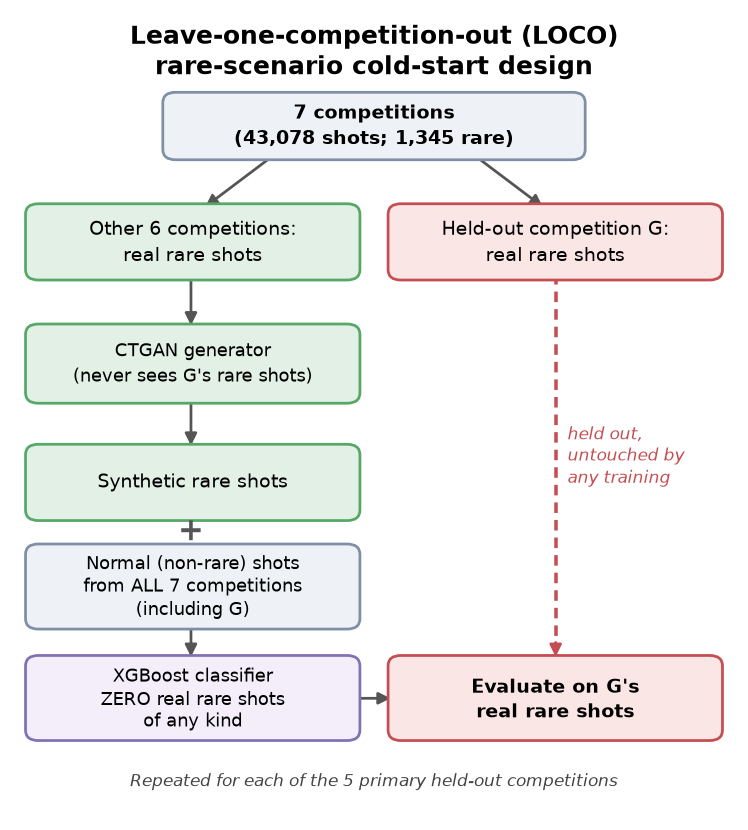
\includegraphics[width=0.78\linewidth]{fig_loco_pipeline_diagram.png}
\caption{The LOCO rare-scenario cold-start design. The held-out competition's rare shots reach neither the generator nor the classifier; its \emph{normal} shots remain in training, making this a cold start for the rare scenario rather than for the whole competition.}
\label{fig:pipeline}
\end{figure}

%=======================================================================
\section{Results}
\label{sec:results}

\subsection{Baselines and the augmentation-vs-baseline effect}
Averaged across the eight match-grouped splits, Baseline A achieves test-set log loss $0.4265\pm0.0344$, Brier $0.1402\pm0.0143$, AUC $0.7767\pm0.0480$, and calibration error $0.2064\pm0.0235$ (Table~\ref{tab:aggregate}). Both augmentation methods modestly outperform it, but not with equal statistical support. CTGAN's validation-selected configuration reaches log loss $0.4225\pm0.0350$, an improvement of $\Delta=-0.0041$ (95\% CI $[-0.0070,-0.0009]$; $d_z=-0.852$; $t$-test $p=0.047$; exact permutation $p=0.047$). The two tests agree closely, but the effect is small and sits near the conventional threshold, so it is best read as a consistent-but-modest improvement whose interval excludes zero rather than a decisive result. SMOTE reaches $0.4206\pm0.0336$, a nominally larger improvement ($\Delta=-0.0059$) that is \emph{not} statistically supported (95\% CI $[-0.0200,0.0082]$; $p=0.449$; permutation $p=0.50$). SMOTE's larger average edge is driven by a subset of favorable splits -- its selected ratio ranges 1\%--1{,}000\% across splits -- not by a consistent effect.

%-----------------------------------------------------------------------
\begin{table*}[!t]
\centering
\caption{Eight-Split Match-Grouped Aggregate (mean of per-split means $\pm$ std across splits; validation-selected ratio, held-out test evaluation)}
\label{tab:aggregate}
\scriptsize
\begin{tabular}{lccccl}
\toprule
Config. & Log Loss & Brier & AUC & Calib.\ Err. & $\Delta$ Log Loss vs.\ Baseline A (95\% CI; $p$; $p_{\text{perm}}$) \\
\midrule
Baseline A & $0.4265\pm0.0344$ & $0.1402\pm0.0143$ & $0.7767\pm0.0480$ & $0.2064\pm0.0235$ & -- \\
CTGAN (val.-selected) & $0.4225\pm0.0350$ & $0.1379\pm0.0147$ & $0.7785\pm0.0479$ & $0.2068\pm0.0254$ & $-0.0041$ \ [$-0.0070,-0.0009$] \ $p=0.047$ \ $p_{\text{perm}}=0.047$ \\
SMOTE (val.-selected) & $0.4206\pm0.0336$ & $0.1359\pm0.0126$ & $0.7566\pm0.0655$ & $0.1887\pm0.0274$ & $-0.0059$ \ [$-0.0200,0.0082$] \ $p=0.449$ \ $p_{\text{perm}}=0.500$ \\
\bottomrule
\end{tabular}

\vspace{2pt}
\raggedright\scriptsize CTGAN selected ratios across splits: 1\%, 1\%, 1\%, 10\%, 10\%, 20\%, 40\%, 80\%. SMOTE: 1\%, 10\%, 50\%, 100\%, 700\%, 800\%, 1{,}000\%, 1{,}000\%. CTGAN-vs-SMOTE paired across splits: mean diff.\ $+0.0018$, $t=0.278$, $p=0.789$, exact permutation $p=0.750$ (not significant).
\end{table*}

\subsection{CTGAN vs.\ SMOTE: an unstable comparison}
\label{sec:instability}
Which augmentation method wins standard rare-scenario augmentation is a methodologically important null result. Under the original shot-level split, SMOTE reached significance against a real-data baseline at the majority of eighteen ratios while CTGAN rarely did. Switching to a single match-grouped split reversed this completely: CTGAN reached significance at all eighteen ratios and SMOTE at none. A three-additional-seed robustness check at four representative ratios found the reversal itself unstable -- CTGAN beat SMOTE in only 4 of 12 seed$\times$ratio combinations -- motivating the eight-split study. Its result: CTGAN wins 3 of 8 splits, SMOTE wins 5 of 8 (Fig.~\ref{fig:splitdist}), and the paired difference is not statistically supported by either test (Table~\ref{tab:aggregate}). No stable ``best ratio'' survives either: CTGAN's selected ratio spans 1\%--80\%, SMOTE's 1\%--1{,}000\%.

%-----------------------------------------------------------------------
\begin{figure}[!t]
\centering
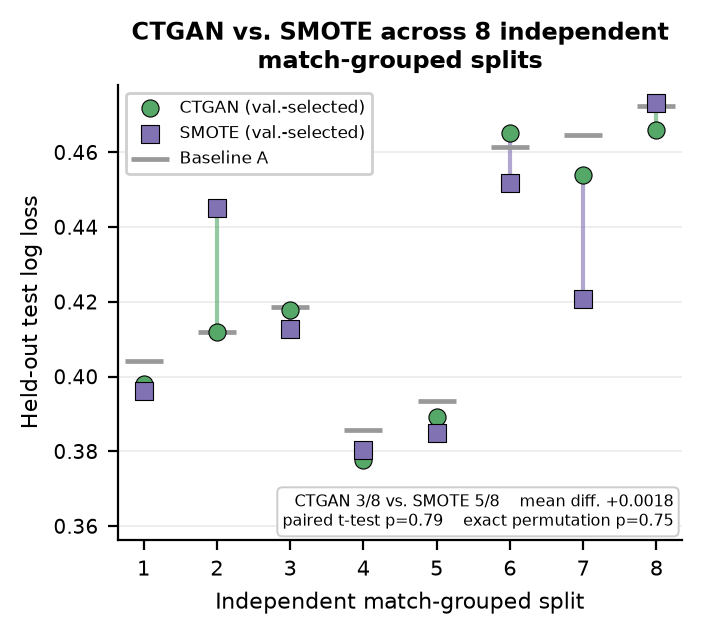
\includegraphics[width=\linewidth]{fig_splitdist_ctgan_smote.png}
\caption{CTGAN vs.\ SMOTE final (validation-selected-ratio) test log loss across eight independently-drawn match-grouped splits. Neither method wins consistently, and the paired difference across splits is not statistically supported. Markers are paired within each split; gray horizontal segments indicate the split-specific baseline.}
\label{fig:splitdist}
\end{figure}

\subsection{LOCO rare-scenario cold-start transfer}
\label{sec:locoresults}
This is the paper's central finding (Table~\ref{tab:loco}, Fig.~\ref{fig:loco}). Averaged across five held-out competitions, the cold-start model $C_G$ -- trained on zero real rare shots, using only CTGAN-synthesized rare shots from a generator that never saw the held-out competition's rare shots -- achieves macro-averaged log loss $0.3546\pm0.0492$, Brier $0.1098\pm0.0186$, AUC $0.7705\pm0.0340$, and calibration error $0.1463\pm0.0209$ at 5\% synthetic augmentation, against the fair baseline $B_G$ at $0.4267$, $0.1403$, $0.7969$, and $0.2120$. This is a 31.0\% relative calibration-error improvement, 95\% CI $[23.6\%,39.3\%]$ (two-stage bootstrap), fold-level Cohen's $d_z=-3.562$ ($t=-7.965$, $p=0.0013$). The improvement is consistent \emph{in direction} across every individual competition (22.2\%--44.4\%); direction, not per-competition significance, is what the exact paired permutation test registers, and because all five folds improve -- the most extreme attainable outcome -- it returns $p=0.0625$, the smallest two-sided value reachable at $N=5$ ($2/2^5$). That floor lies above 0.05 by construction, so the permutation test does not cross $\alpha=0.05$ and is not claimed as significant. Given the small number of folds, the bootstrap interval and paired $t$-test provide the primary quantitative evidence, while the exact permutation test is reported as a conservative sensitivity analysis. Five competitions remains a small basis for population-level generalization.

\subsection{What the synthetic data actually contributes}
\label{sec:modeln}
The normal-only control $N$ (Table~\ref{tab:loco}) separates two explanations for $C_G$'s gain: genuine synthetic rare-event information, versus the training-distribution change that follows from withholding real rare shots. The headline number decomposes into two stages. First, $B_G\!\to\!N$: the control alone reaches macro calibration error $0.1704$, already 19.6\% better than $B_G$, so roughly two-thirds of the 31.0\% total is obtained without any rare-scenario signal at all. Second, $N\!\to\!C_G$: the synthetic condition adds a further 14.2\% macro-average improvement to reach $0.1463$, with improvement in all five folds, though the per-fold gains vary widely (England 18.7\%, France 12.0\%, Germany 1.4\%, Italy 30.6\%, Spain 7.8\%; $t=2.832$, $p=0.047$; exact permutation $p=0.0625$, again at the $N=5$ floor). The combined $B_G\!\to\!C_G$ difference is the 31.0\% headline. The precise reading is therefore narrower than ``synthetic rare shots deliver a 31\% calibration gain'': most of that margin reflects the training-distribution change, and the synthetic condition provides an additional, smaller improvement on top of it.

Because the three conditions have different training-set class compositions and \texttt{scale\_pos\_weight} is otherwise recomputed per training set, this decomposition could in principle be a reweighting artifact. Re-running all three conditions at the 5\% ratio with the weight held fixed at the normal-only training set's value leaves it essentially unchanged: macro calibration $B_G$ $0.2116$, $N$ $0.1704$, $C_G$ $0.1455$, giving $B_G\!\to\!N$ 19.5\% and $N\!\to\!C_G$ 14.6\%, positive in 5/5 folds ($t=4.804$, $p=0.009$). The additional synthetic-condition improvement therefore remains positive under fixed class weighting and is not attributable to the class-weight change.

Holm-adjusted across all six ratios, the $C_G$-vs-$B_G$ improvement is significant from 5\% through 50\% (adjusted $p\le0.032$) but not at 100\% (adjusted $p=0.207$), where the bootstrap interval also includes zero ($[-2.0\%,19.5\%]$). Fig.~\ref{fig:loco2} shows this dose-response: the benefit concentrates at low ratios and decays monotonically in the macro-average. AUC falls by roughly 0.03 relative to $B_G$; the result is consistent with improved calibration of the probability scale, even where the cold-start model cannot fully reproduce the held-out competition's discriminative structure. For a model informing probability estimates for a competition with no rare-shot history, calibration is the more decision-relevant of the two. A supplementary fold merging World\_Cup and European\_Championship (61 shots, 4 goals) shows the same direction at 5\% (14.2\% calibration improvement) with substantially wider variance, excluded from the primary aggregate for low-positive-count fragility rather than as a contradicting result.

%-----------------------------------------------------------------------
\begin{table}[!t]
\centering
\caption{LOCO Rare-Scenario Cold-Start at 5\% Synthetic Ratio: fair baseline $B_G$, normal-only control $N$, and cold-start model $C_G$}
\label{tab:loco}
\scriptsize
\setlength{\tabcolsep}{2.4pt}
\begin{tabular}{lccccccc}
\toprule
 & & \multicolumn{2}{c}{Brier} & \multicolumn{3}{c}{Calibration Error} & \\
\cmidrule(lr){3-4}\cmidrule(lr){5-7}
Fold & $n$ (goals) & $B_G$ & $C_G$ & $B_G$ & $N$ & $C_G$ & Impr.\ \\
\midrule
England & 271 (26) & 0.1385 & 0.1073 & 0.2198 & 0.1769 & 0.1439 & 34.5\% \\
France & 282 (19) & 0.1343 & 0.1056 & 0.2146 & 0.1804 & 0.1587 & 26.0\% \\
Germany & 208 (22) & 0.1577 & 0.1336 & 0.2214 & 0.1748 & 0.1723 & 22.2\% \\
Italy & 267 (18) & 0.1316 & 0.0832 & 0.2099 & 0.1683 & 0.1168 & 44.4\% \\
Spain & 256 (30) & 0.1393 & 0.1191 & 0.1941 & 0.1518 & 0.1399 & 27.9\% \\
\midrule
\textbf{Macro} & \textbf{1{,}284 (115)} & \textbf{0.1403} & \textbf{0.1098} & \textbf{0.2120} & \textbf{0.1704} & \textbf{0.1463} & \textbf{31.0\%} \\
\bottomrule
\end{tabular}

\vspace{2pt}
\raggedright\scriptsize Macro rows are \emph{unweighted} means across the five competitions. $C_G$ values are means over $N=5$ runs; $B_G$ and $N$ are deterministic. ``Impr.'' is $C_G$'s relative calibration improvement over $B_G$ (95\% CI $[23.6\%,39.3\%]$ at macro). Macro log loss: $B_G$ 0.4267, $N$ 0.3810, $C_G$ 0.3546. \textbf{Macro decomposition (calibration):} $B_G\!\to\!N$ 19.6\%, $N\!\to\!C_G$ 14.2\%, $B_G\!\to\!C_G$ 31.0\% -- all three are macro-average quantities; per-fold $N\!\to\!C_G$ gains range 1.4\%--30.6\%.
\end{table}

%-----------------------------------------------------------------------
\begin{figure}[!t]
\centering
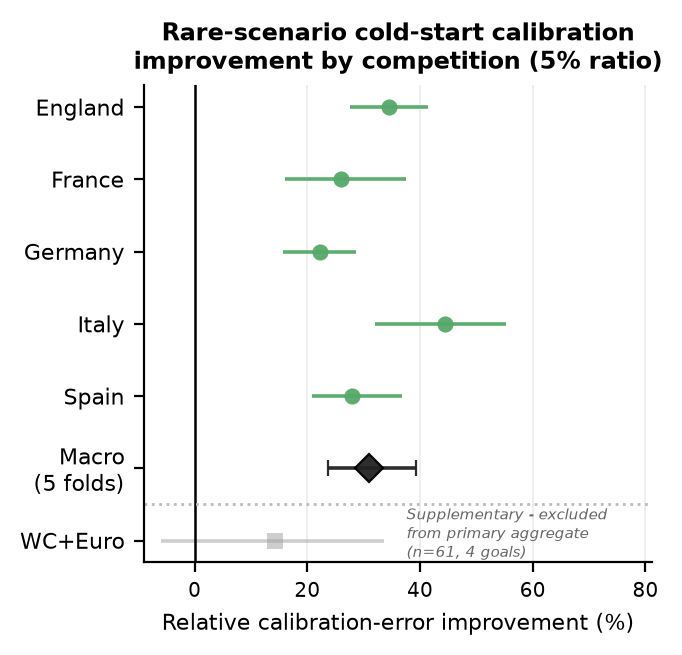
\includegraphics[width=\linewidth]{fig_loco_per_fold.png}
\caption{Rare-scenario cold-start calibration improvement over the fair baseline $B_G$ at 5\% synthetic ratio, per held-out competition, with 95\% bootstrap CIs. The diamond denotes the unweighted macro-average across the five primary LOCO folds.}
\label{fig:loco}
\end{figure}

%-----------------------------------------------------------------------
\begin{figure}[!t]
\centering
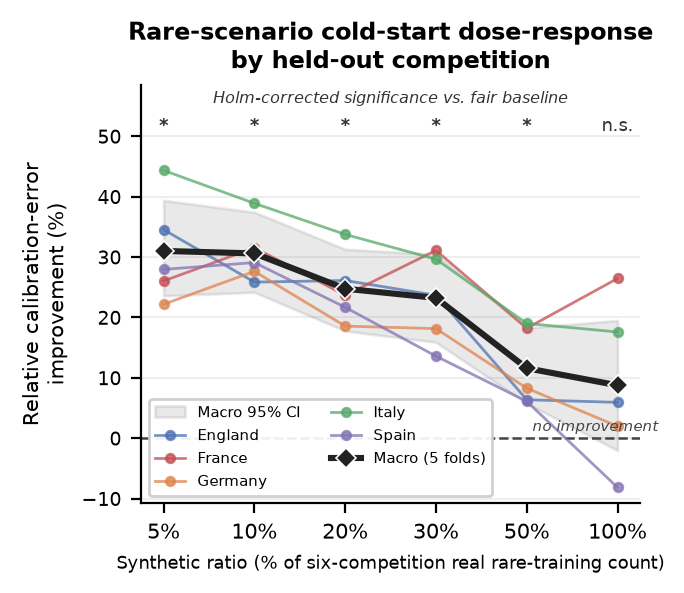
\includegraphics[width=\linewidth]{fig_loco_dose_response.png}
\caption{Dose-response across all six tested synthetic ratios. The macro-averaged improvement decays with ratio and loses Holm-corrected significance at 100\%.}
\label{fig:loco2}
\end{figure}

\subsection{Supporting observations}
Feature importance rankings (by XGBoost gain) remain stable across baseline and augmented configurations, with distance and angle dominant throughout, consistent with Mead et al.~\cite{mead2023expected}. Marginal distributional similarity, as measured here by pressure-index JS divergence, did not reliably predict downstream utility: CTGAN's \texttt{pressure\_index} had the lower JS divergence of the two methods (0.1078 vs.\ 0.1406), yet this did not translate into a stable downstream advantage once evaluated across splits.

%=======================================================================
\section{Conclusion}
A leave-one-competition-out design in which neither the CTGAN generator nor the downstream classifier sees any real rare shot from the held-out competition improves rare-scenario calibration over a leakage-free baseline in all five competitions tested. The effect has a bootstrap 95\% CI excluding zero at 5\% augmentation and remains significant under Holm-adjusted paired t-tests across five of six tested ratios, although the exact five-fold permutation test does not reach 0.05. A normal-only control shows roughly two-thirds of that gain follows from withholding real rare shots rather than from synthesis; the synthetic condition adds a further 14.2\% macro-average improvement over the control, with improvement in all five folds and per-fold gains varying widely, and remains positive under fixed class weighting. Separately, the CTGAN-vs-SMOTE ranking reversed between splitting schemes and is not statistically supported across eight splits, so neither method should be reported as winning. Five competitions and eight splits remain small bases for population-level inference, and both headline claims should be read as well-quantified within this dataset rather than established across football data at large.

\subsection{Reproducibility Statement}
Code, split assignments, result artifacts, and analysis seeds are retained for reproducibility; all headline estimates are based on the eight grouped splits and five LOCO folds described above. All XGBoost models use a fixed seed (42) with a distinct seed per augmentation-sampling run, and every ratio/fold/split combination is evaluated over $N=5$ independent sampling runs.

%=======================================================================
\bibliographystyle{IEEEtran}
\bibliography{bibtex}

\end{document}
